\documentclass[10pt]{article}

\usepackage{fullpage}
\usepackage{setspace}
\usepackage{parskip}
\usepackage{titlesec}
\usepackage{placeins}
\usepackage{xcolor}
\usepackage{lineno}





\PassOptionsToPackage{hyphens}{url}
\usepackage[colorlinks = true,
            linkcolor = blue,
            urlcolor  = blue,
            citecolor = blue,
            anchorcolor = blue]{hyperref}
\usepackage{etoolbox}
\makeatletter
\patchcmd\@combinedblfloats{\box\@outputbox}{\unvbox\@outputbox}{}{%
  \errmessage{\noexpand\@combinedblfloats could not be patched}%
}%
\makeatother


\usepackage{natbib}




\renewenvironment{abstract}
  {{\bfseries\noindent{\abstractname}\par\nobreak}\footnotesize}
  {\bigskip}

\renewenvironment{quote}
  {\begin{tabular}{|p{13cm}}}
  {\end{tabular}}

\titlespacing{\section}{0pt}{*3}{*1}
\titlespacing{\subsection}{0pt}{*2}{*0.5}
\titlespacing{\subsubsection}{0pt}{*1.5}{0pt}


\usepackage{authblk}


\usepackage{graphicx}
\usepackage[space]{grffile}
\usepackage{latexsym}
\usepackage{textcomp}
\usepackage{longtable}
\usepackage{tabulary}
\usepackage{booktabs,array,multirow}
\usepackage{amsfonts,amsmath,amssymb}
\providecommand\citet{\cite}
\providecommand\citep{\cite}
\providecommand\citealt{\cite}
% You can conditionalize code for latexml or normal latex using this.
\newif\iflatexml\latexmlfalse
\providecommand{\tightlist}{\setlength{\itemsep}{0pt}\setlength{\parskip}{0pt}}%

\AtBeginDocument{\DeclareGraphicsExtensions{.pdf,.PDF,.eps,.EPS,.png,.PNG,.tif,.TIF,.jpg,.JPG,.jpeg,.JPEG}}

\usepackage[utf8]{inputenc}
\usepackage[english]{babel}






% Edit this header.tex file to include frontmatter definitions and global macros

% Add here any LaTeX packages you would like to load in all document blocks
% \usepackage{xspace}
\usepackage{authblk}

\author[1]{Mark Juers}
\affil[1]{Indiana University}
% Add here any LaTeX macros you would like to load in all document blocks
% \def\example{This is an example macro.}
\setcounter{secnumdepth}{2}


% -----

\iflatexml
% Add here any LaTeXML-specific commands

% -----

\else
% Add here any export style-specific LaTeX commands. These will only be loaded upon document export. 
% \paperfield{Subject domain of my document}
% \keywords{keyword1, keyword2}
% \corraddress{Author One PhD, Department, Institution, City, State or Province, Postal Code, Country}
% \fundinginfo{Funder One, Funder One Department, Grant/Award Number: 123456.}
\fi


\begin{document}

\title{Test document}



\author[1]{Mark Juers}%
\affil[1]{Affiliation not available}%


\vspace{-1em}



  \date{\today}


\begingroup
\let\center\flushleft
\let\endcenter\endflushleft
\maketitle
\endgroup





\selectlanguage{english}
\begin{abstract}
An abstract.%
\end{abstract}%




\section*{A heading}

{\label{850151}}

\subsection*{Another heading}

{\label{367935}}

\hyperref[csl:1]{(Ebert, 2013)}

\hyperref[csl:1]{(Ebert, 2013)}

\hyperref[csl:1]{(Ebert, 2013)}

Figure {\ref{286335}}

Eq~{\ref{eq:eq1}}

An inline equation:~\(\int_0^xf\left(t\right)\mathrm{d}t\). And a display equation.

\begin{equation}
\label{eq:eq1}
\int_0^x f(t) \mathrm{d}t
\end{equation}

Some troublesome dollar signs: \$100, \$200, \$300

Section~{\ref{850151}}

\section*{Some markdown}\label{some-markdown}

Once, there was a cuttlefish, who we'll call \emph{Sepia apama}. Now,
some math: \(a + b = c\).\selectlanguage{english}
\begin{figure}[h!]
\begin{center}
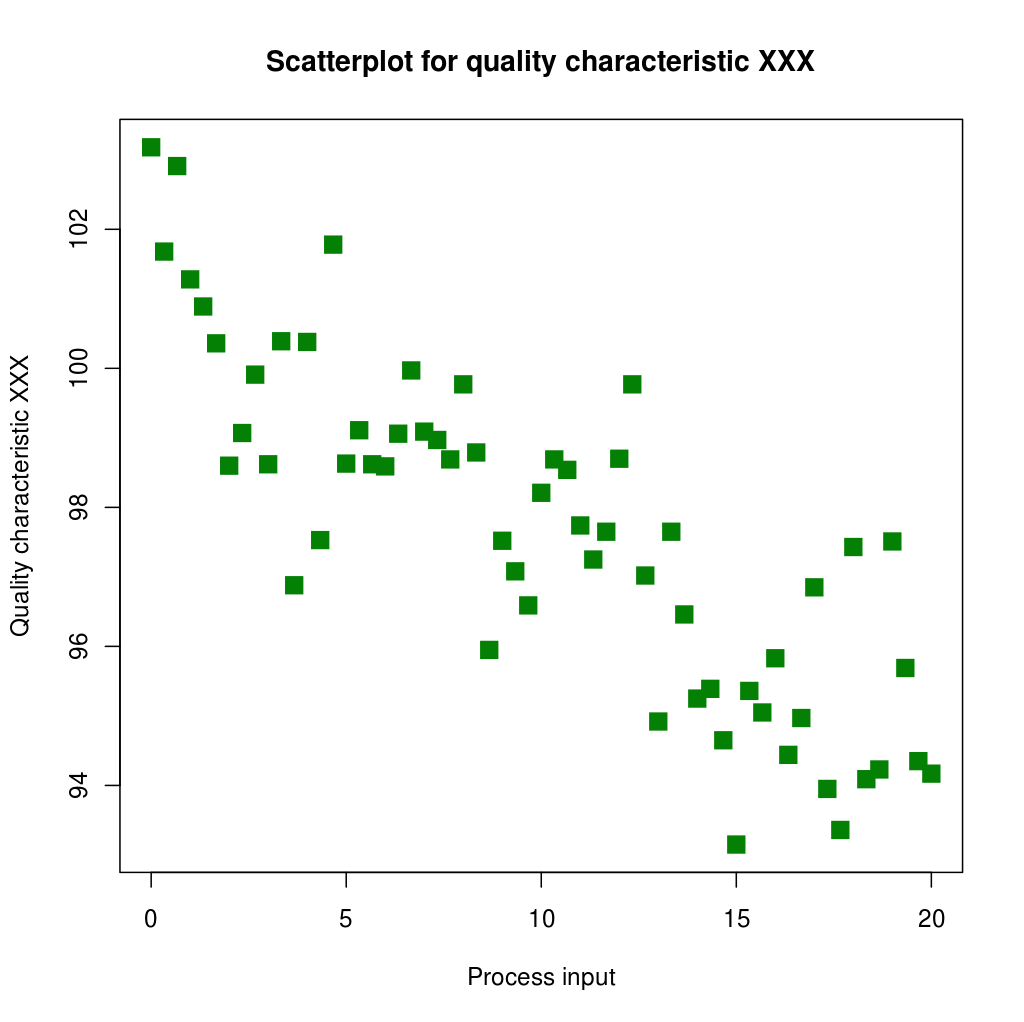
\includegraphics[width=0.70\columnwidth]{figures/scatterplot/scatterplot}
\caption{{A scatterplot by By DanielPenfield - Own work, CC BY-SA 3.0,
\url{https://commons.wikimedia.org/w/index.php?curid=9402369}.
{\label{286335}}%
}}
\end{center}
\end{figure}

\selectlanguage{english}
\FloatBarrier
\section*{References}\sloppy
\phantomsection
\label{csl:1}Ebert, D. (2013). {The epidemiology and evolution of symbionts with mixed-mode transmission}. \textit{Annual Review of Ecology, Evolution, and Systematics}, \textit{44}(1), 623–643. \url{https://doi.org/10.1146/annurev-ecolsys-032513-100555}

\end{document}

